% TikZ verwendet Grad; 4*pi*x im Bogenmass entspricht 720*x Grad.
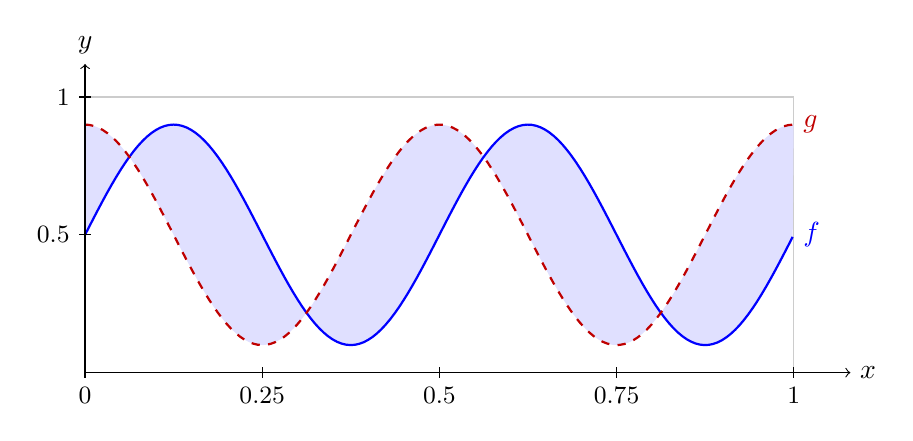
\begin{tikzpicture}[x=9cm, y=3.5cm]
    \draw[gray!40] (0,0) rectangle (1,1);
    \path[fill=blue!12]
        plot[domain=0:1, samples=161] (\x,{0.5+0.4*sin(720*\x)})
        -- plot[domain=1:0, samples=161] (\x,{0.5+0.4*cos(720*\x)})
        -- cycle;
    \draw[blue, thick] plot[domain=0:1, samples=161]
        (\x,{0.5+0.4*sin(720*\x)});
    \draw[red!75!black, thick, dashed] plot[domain=0:1, samples=161]
        (\x,{0.5+0.4*cos(720*\x)});
    \draw[->] (0,0) -- (1.08,0) node[right] {$x$};
    \draw[->] (0,0) -- (0,1.12) node[above] {$y$};
    \foreach \x in {0,0.25,0.5,0.75,1}
        \draw (\x,0.02) -- (\x,-0.02) node[below] {\small $\x$};
    \foreach \y in {0.5,1}
        \draw (0.008,\y) -- (-0.008,\y) node[left] {\small $\y$};
    \node[blue, right] at (1,0.5) {$f$};
    \node[red!75!black, right] at (1,0.9) {$g$};
\end{tikzpicture}
